In this section, the user is prompted to the login page. The user have to use the existing login information to login and access to the system account. 

\subsection{Input Validation}
This section validates the inputs given for the login information. This sub system checks if the user ID and Password is already registered in the system or not. Only the previously registered account information is validated and given access.

\begin{figure}[h!]
	\centering
 	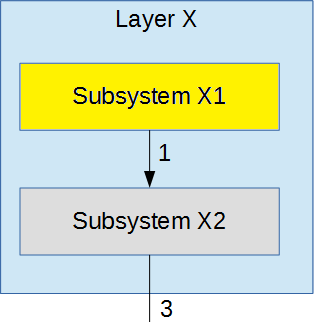
\includegraphics[width=0.60\textwidth]{images/subsystem}
 \caption{Example subsystem description diagram}
\end{figure}

\subsubsection{Assumptions}
Following assumptions are made for this system:
\begin{itemize}
    \item Inventory app is already installed on the users cellphone.
    \item User clicked on the Login button after giving Username and Password information.
\end{itemize}

\subsubsection{Responsibilities}
Following are the responsibilities of this sub system:
\begin{itemize}
    \item This sub system must check if the user inputs (Username and Password) is already registered in the system. If the information is already in the system, then it will allow the user to access their account.
\end{itemize}

\subsubsection{Subsystem Interfaces}
Each of the inputs and outputs for the subsystem are defined here. Create a table with an entry for each labelled interface that connects to this subsystem. For each entry, describe any incoming and outgoing data elements will pass through this interface.

\begin {table}[H]
\caption {Subsystem interfaces} 
\begin{center}
    \begin{tabular}{ | p{1cm} | p{6cm} | p{3cm} | p{3cm} |}
    \hline
    ID & Description & Inputs & Outputs \\ \hline
    \#xx & Description of the interface/bus & \pbox{3cm}{input 1 \\ input 2} & \pbox{3cm}{output 1}  \\ \hline
    \#xx & Description of the interface/bus & \pbox{3cm}{N/A} & \pbox{3cm}{output 1}  \\ \hline
    \end{tabular}
\end{center}
\end{table}

\subsection{Subsystem 2}
Repeat for each subsystem

\subsection{Subsystem 3}
Repeat for each subsystem

